

\chapter{Frequently Asked Questions}\label{frequently-asked-questions}

\FILENAME

\section{Appliances}\label{appliances}

\subsection{What is an appliance?}\label{what-is-an-appliance}

An appliance is an application packaged together with the environment
that this application requires. For example, an appliance can consists
of the operating system, libraries and tools used by the application,
configuration features such as environment variable settings, and the
installation of the application itself. Examples of appliances might
include a KVM virtual machine image, a Docker image, or a bare metal
image. Chameleon appliance refers to bare metal images that can be
deployed on the Chameleon testbed. Since an appliance captures the
experimental environment exactly, it is a key element of
reproducibility; publishing an appliance used to obtain experimental
results will go a long way to allowing others to reproduce and build on
your research easily.

To deploy distributed applications on several~Chameleon instances,
complex appliances combine an~image and a~template describing how the
cluster should be configured and contextualized. You can read more about
them in the
\href{https://www.chameleoncloud.org/docs/complex-appliances/}{Complex
Appliances documentation}.

\subsection{What is the Appliance Catalog?}\label{what-is-the-chameleon-appliance-catalog}

\href{https://www.chameleoncloud.org/appliances/}{The Chameleon
Appliance Catalog}~is a repository that allows users to discover,
publish, and share appliances. The appliance catalog contains useful
images of both bare metal and virtual machine appliances supported by
the Chameleon team as well appliances contributed by users.

\subsection{How do I publish an appliance in the Appliance Catalog?}\label{how-do-i-publish-an-appliance-in-the-chameleon-appliance-catalog}

The new Appliance Catalog allows you to easily publish and share your
own appliances so that others can discover them and use them either to
reproduce the research of others or as a basis for their own research.
~Before creating your own appliance it is advisable to review other
appliances on
the~\href{https://www.chameleoncloud.org/appliances/}{Chameleon
Appliance Catalog}~in order to get an idea of the categories you will
want to contribute and what others have done.~

Once you are ready to proceed, an appliance can be contributed to
Chameleon in the following steps:

\begin{enumerate}
\tightlist
\item
  Create the appliance itself. You may want to test it as well as give
  some thought to what support you are willing to provide for the
  appliance (e.g., if your group developed and supports a software
  package, the appliance may be just a new way of packaging the software
  and making it available, in which case your standard support channels
  may be appropriate for the appliance as well).
\item
  Upload the appliance to the Chameleon Image Repository (Glance) and
  make the image public. In order to enter the appliance into the
  Catalog you will be asked to provide the Glance ID for the image.
  These IDs are per-cloud, so that there are three options right now:
  bare metal/CHI at University of Chicago, bare metal/CHI at TACC, and
  OpenStack/KVM at TACC. You will need to provide at least one
  appliance, but may want to provide all three.
\item
  Go to
  the~\href{https://www.chameleoncloud.org/appliances/create/}{Appliance
  Catalog Create Appliance web form}, fill out, and submit the form. Be
  prepared to provide the following information: a descriptive name
  (this sometimes requires some thought!), author and support contact,
  version, and an informative description. The description is a very
  important part of the appliance record; others will use it to evaluate
  if the appliance contains tools they need for their research so it
  makes sense to prepare it carefully. To make your description
  effective you may want to think of the following questions: what does
  the appliance contain? what are the specific packages and their
  versions? what is it useful for? where can it be deployed and/or what
  restrictions/limitations does it have? how should users connect to it
  / what accounts are enabled?
\end{enumerate}

If you are adding a complex appliance, skip the image ID fields and
enter your template instead in the dedicated text box.

As always, if you encounter any problems or want to share with us
additional improvements we should do to the process, please don't
hesitate to~\href{https://www.chameleoncloud.org/help/}{submit a
ticket}.~

\subsection{How can I manage an appliance on Appliance
Catalog?}\label{how-can-i-manage-an-appliance-on-chameleon-appliance-catalog}

If you are the owner of the appliance,~you can edit~the appliance
data,~such as the description or the support information. Browse to the
appliance that you want to edit and view its Details page. At the top
right of the page is an Edit button. You will be presented with the same
web form as when creating the appliance, pre-filled with the appliances
current information. Make changes as necessary and click Save at the
bottom of the page.

And finally, you can delete appliances you had made available.~{Browse
to the appliance that you want to delete~and click Edit on the
Appliance~Details page. At the bottom of the page is a Delete button.
You will be asked to confirm once more that you do want to delete this
appliance}. After confirming, the appliance will be removed and no
longer listed on the Appliance Catalog.

\subsection{Why are there different image IDs  for the same
appliance?}\label{why-are-there-different-image-ids-for-kvmtacc-chitacc-and-chiuc-for-the-same-appliance}

The three clouds forming the Chameleon testbed are fully separated, each
having its own Glance image repository. The same appliance
image~uploaded to the three clouds will produce three different image
IDs.

In addition, it is sometimes needed to customize an appliance image for
each site, resulting in slightly different image files.

\subsection{Can I use another operating system on bare-metal?}\label{can-i-useubuntudebian-oranother-operating-system-rather-than-centos-on-bare-metal}

The recommended appliance for Chameleon is CentOS 7~(supported by
Chameleon staff), or appliances built on top of it.\\
These appliances provide~Chameleon-specific customizations, such as
login using the~cc account, the~cc-checks utility to verify hardware
against our resource registry, gathering of metrics, etc.

Since 2016, we also provide and~support Ubuntu 14.04 and
16.04~appliances with the same functionality.

\section{Bare Metal Troubleshooting}\label{bare-metal-troubleshooting}

\subsection{Why are my Bare Metal instances failing to
launch?}\label{why-are-my-bare-metal-instances-failing-to-launch}

The Chameleon Bare Metal clouds require users to reserve resources
before allowing them to launch instances. Please follow the
\href{https://www.chameleoncloud.org/docs/bare-metal/}{documentation}
and make sure that:

\begin{enumerate}
\item
  You have created a lease and it has started (the associated
  reservation is shown as \textbf{Active})
\item
  You have selected your reservation in the \textbf{Launch Instance}
  panel
\end{enumerate}

If you still cannot start instances, please
\href{https://www.chameleoncloud.org/user/help/}{open a ticket with our
help desk}.

\section{OpenStack KVM Troubleshooting}\label{openstack-kvm-troubleshooting}

\subsection{Why are my OpenStack KVM instances failing to
launch?}\label{why-are-my-openstack-kvm-instances-failing-to-launch}

If you get an error stating that~\textbf{No valid host was found}, it
might be caused by a lack of resources in the cloud. The Chameleon staff
continuously monitors the utilization of the testbed, but there might be
times when no more resources are available. If the error persists,
please~\href{https://www.chameleoncloud.org/user/help/}{open a ticket
with our help desk}.

\subsection{Why can't I ping or SSH to my
instance?}\label{why-cant-i-ping-or-ssh-to-my-instance}

While the possibility that the system is being taking over by nanites
should not be discounted too easily, it is always prudent to first
check~for the~following issues:

\begin{itemize}
\item
  Do you have a floating IP associated with your instance?~By default,
  instances do not have publicly-accessible IP addresses assigned. See
  the \textbf{Managing Virtual Machine Instances} section in the
  \href{https://www.chameleoncloud.org/docs/user-guides/openstack-kvm-user-guide/}{User
  Guide}.
\item
  Does your security group allow incoming ICMP (e.g. ping) traffic?~By
  default, firewall rules do not allow ping to your instances. If you
  wish to enable it, see the \textbf{Firewall (Access Security)} section
  in the
  \href{https://www.chameleoncloud.org/docs/user-guides/openstack-kvm-user-guide/}{User
  Guide}.
\item
  Does your security group allow incoming SSH (TCP port 22) traffic?~By
  default, firewall rules do not allow SSH to your instances. If you
  wish to enable it, see the \textbf{Firewall (Access Security)} section
  in the
  \href{https://www.chameleoncloud.org/docs/user-guides/openstack-kvm-user-guide/}{User
  Guide}.
\end{itemize}

~If none of these~solve~your problem,
please~\href{https://www.chameleoncloud.org/user/help/}{open a ticket
with our help desk}, and send~us the results of the above (and any
evidence of nanites you find as well).

\section{Create your own SSH key pairs}\label{create-your-own-ssh-key-pairs}

The following document describes the procedure on how you can create an
SSH key pair on your Unix, Linux or Windows operating system.

\subsection{For Linux / Mac OS X}\label{for-linux-mac-os-x}

Open a terminal window:

\begin{itemize}
\tightlist
\item
  In a Mac OS X system, click on your launchpad and search for terminal
\item
  In an Ubuntu system you can use the keys Ctrl+Alt+T (for desktop
  version)
\end{itemize}

Access the SSH key pairs directory; {i}n your terminal type the command:

\begin{verbatim}
$ cd ~/.ssh
\end{verbatim}

Create your ssh key pair (public and private keys);~~in~the
\texttt{.ssh} directory, type the command:

\begin{verbatim}
$ ssh-keygen
\end{verbatim}

Press the enter key, then~enter a name for your key.

After completing the previous step, a message stating ``Enter file in
which to save the Key'' will be displayed. Enter the name of your
preference. I will use in this example the name ``sample-key''.{~}Then
press the enter key.

{Then,~}you will be requested to enter a passphrase for your
key.~Entering a passphrase is not necessary, so you can proceed to leave
it blank and press enter.{~}You will receive a message ``Enter same
passphrase again:'' so just leave it blank and press enter.

Since we are still in the \texttt{.ssh} directory, now you can see your
newly created key by typing:

\begin{verbatim}
$ ls
\end{verbatim}

You will see two files:

\begin{itemize}
\tightlist
\item
  sample-key (containing the private key)
\item
  sample-key.pub (containing the public key)
\end{itemize}

Then, provide the public key to your cloud system or individual
instance. To add a key pair in Chameleon,~access one of the resource
dashboards and go the following tabs:

~ ~ Compute \textgreater{} Access and Security \textgreater{} Key Pairs
\textgreater{} Import Key Pair

In this window, you only need to provide a name for your key pair and
paste your public key pair in the ``Public Key'' window. To obtain the
contents of your public key, access your local \texttt{.ssh} directory
through your terminal and use the command:

\begin{verbatim}
$ cat sample-key.pub
\end{verbatim}

Select and copy the contents displayed starting ssh-rsa all the way to
the end. Paste these contents into the ``Public Key'' window~mentioned
earlier.

Whenever you are creating an instance in Chameleon, you will have an
option to select the Public Key you just imported. Once selected, this
public key will be inserted into the instance's
\textasciitilde{}/.ssh/known\_hosts file. When a user attempts to
connect to the instance, the private key provided by the user will be
validated against this public key in the known\_hosts file.

Connect to an instance from your terminal

After you have created a key pair and imported it in
Chameleon, you can connect to~any instance configured with this key
pair. To do so you can use the
command:

\begin{verbatim}
$ ssh -i ~/.ssh/sample-key cc@<instance ip address>
\end{verbatim}

The full process can be viewed in the figure below:

{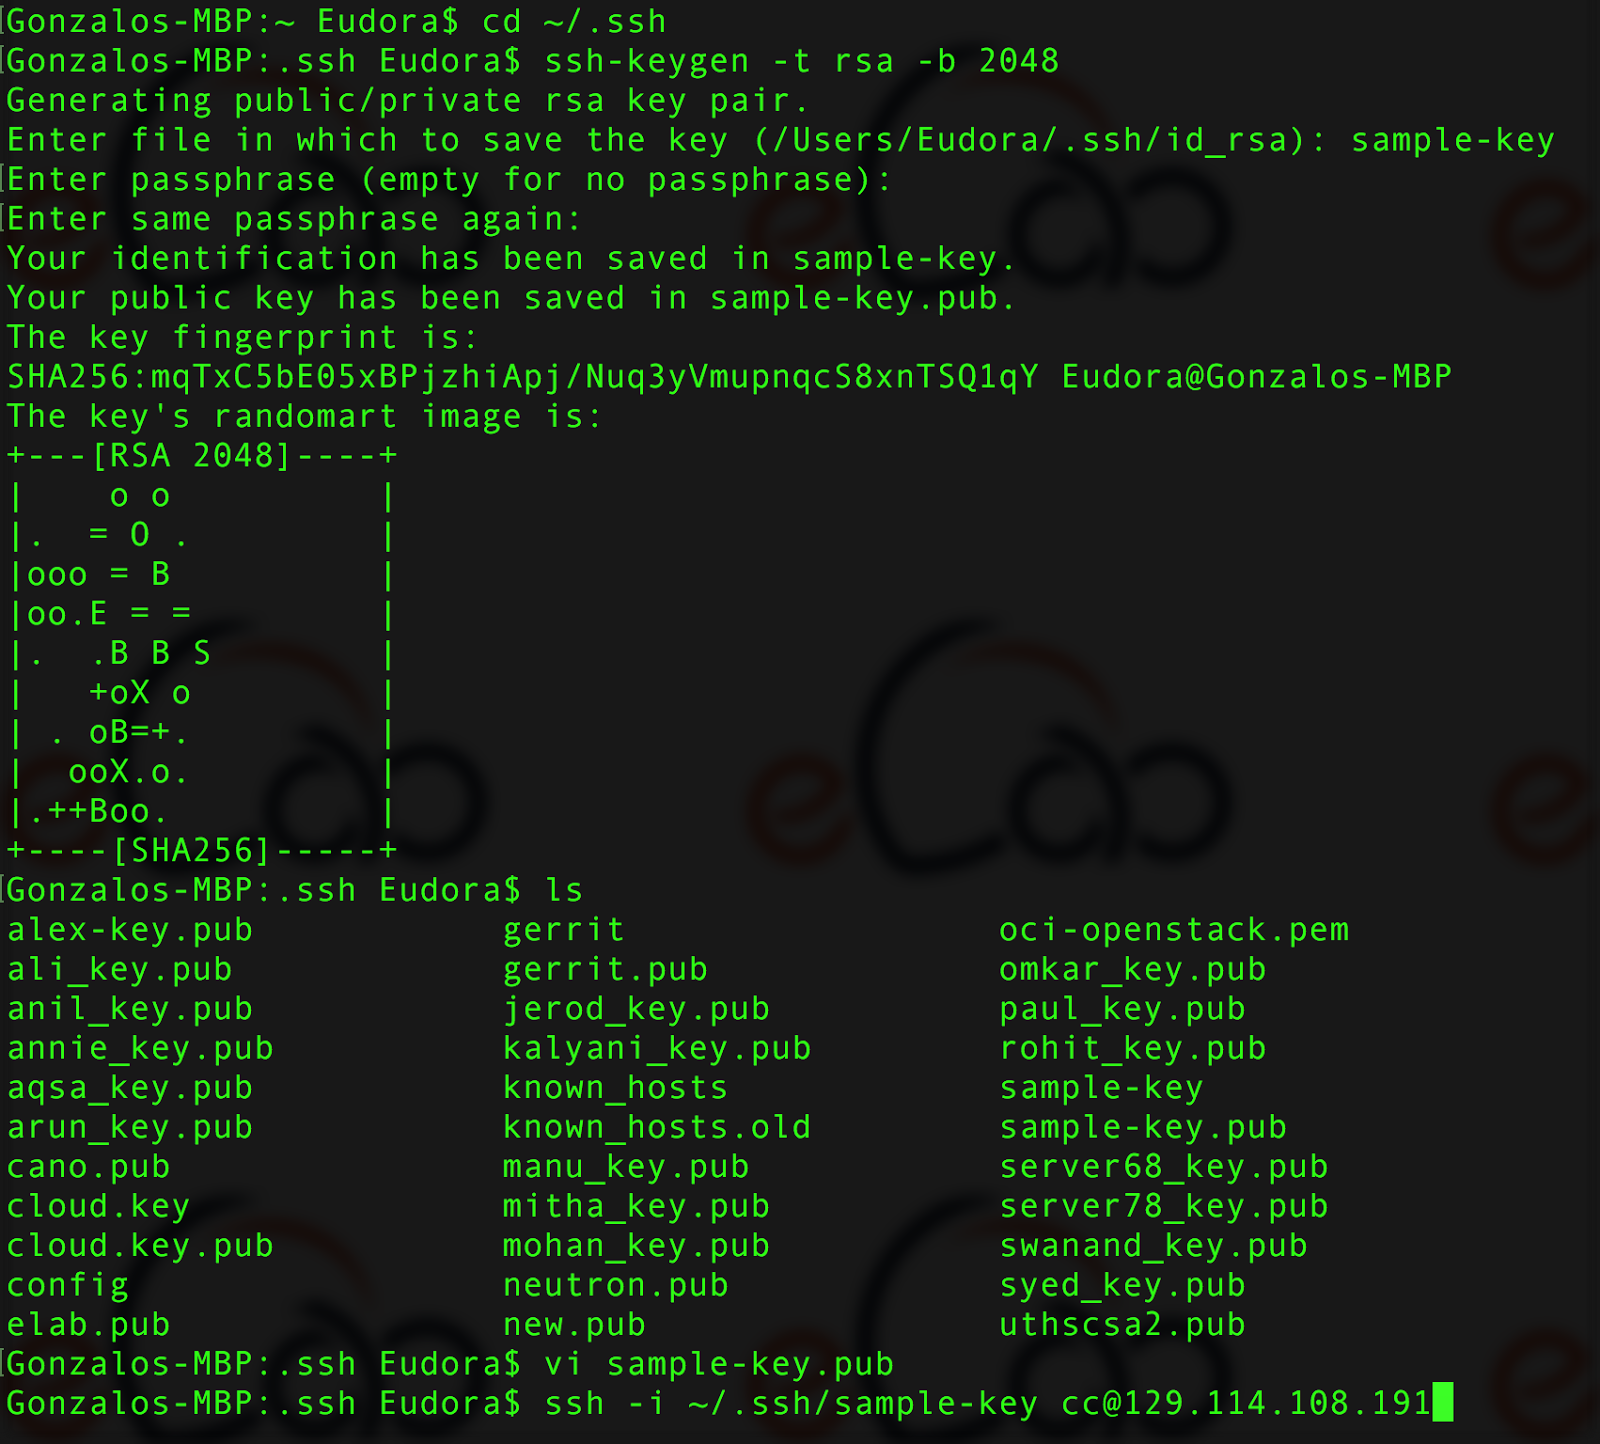
\includegraphics[width=\columnwidth]{images/chameleon/ssh1.png}}

\subsection{PuTTY}

Follow the instructions from Section \ref{S:putty}. 

Before closing this window, select the entire public key and copy it
with ``Control-C''. Please note that everything should be copied,
including ``ssh-rsa''. This will be used when importing the key pair to
Openstack.

At this time, the public key has been created and copied. Now you can
now follow the steps described above (starting with the line ``Provide
the public key to your cloud system or individual instance'') to import
the generated key pair for use with Chameleon!
